\documentclass[Report.tex]{subfiles}
\begin{document}

\chapter{Project Overview}
\section{External Features}
The key components of the application are introduced in this chapter. It is first described from the perspective of the user, highlighting key features that are then explained in terms of the back-end processes required to produce them.

\subsection{Functionality}
The functionality that the application provides to users can be summarised as follows. It can:
\begin{itemize}
\item Accept a search query from the user in the form of a text string,
\item Retrieve up to 20 documents from PubMed based on the user's query,
\item Display geocoded institutional addresses on a map in the browser, and
\item Display concepts related to the documents in the browser.
\end{itemize}

\subsection{User Interface}
The web application is contained within a single page, that is, all POST and GET requests do not result in a redirect, but instead cause the web page to dynamically update and reflect new data. A user starts by entering a text query into a form and pressing a 'search' button adjacent to it. After a duration, the page is updated with the results. Concepts are hierarchically graphed in a visualisation and institutional locations are plotted on a map (Figure \ref{fig:screen1}a). Information from each paper is displayed in a bar above these, allowing the user to cycle through all retrieved papers, also triggering the visualisations to update and emphasise the selected paper (Figure \ref{fig:screen1}b).\newline

\noindent The information bar provides context to the visualisations. Once a paper is selected, the relevant bibliographic information is displayed, the nodes in the concept visualisation are coloured red, and the markers on the Google Map are turned opaque (Figure \ref{fig:screen1}c \& d). Papers can be selected from their geographical elements, or from using the Previous/Next buttons. These can also be triggered using the left and right buttons on the keyboard. The title is hyperlinked to the relevant page on PubMed if the user wants to investigate the citation further.\newpage

\begin{figure}[!]
\begin{center}
	\begin{subfigure}{0.8\textwidth}
		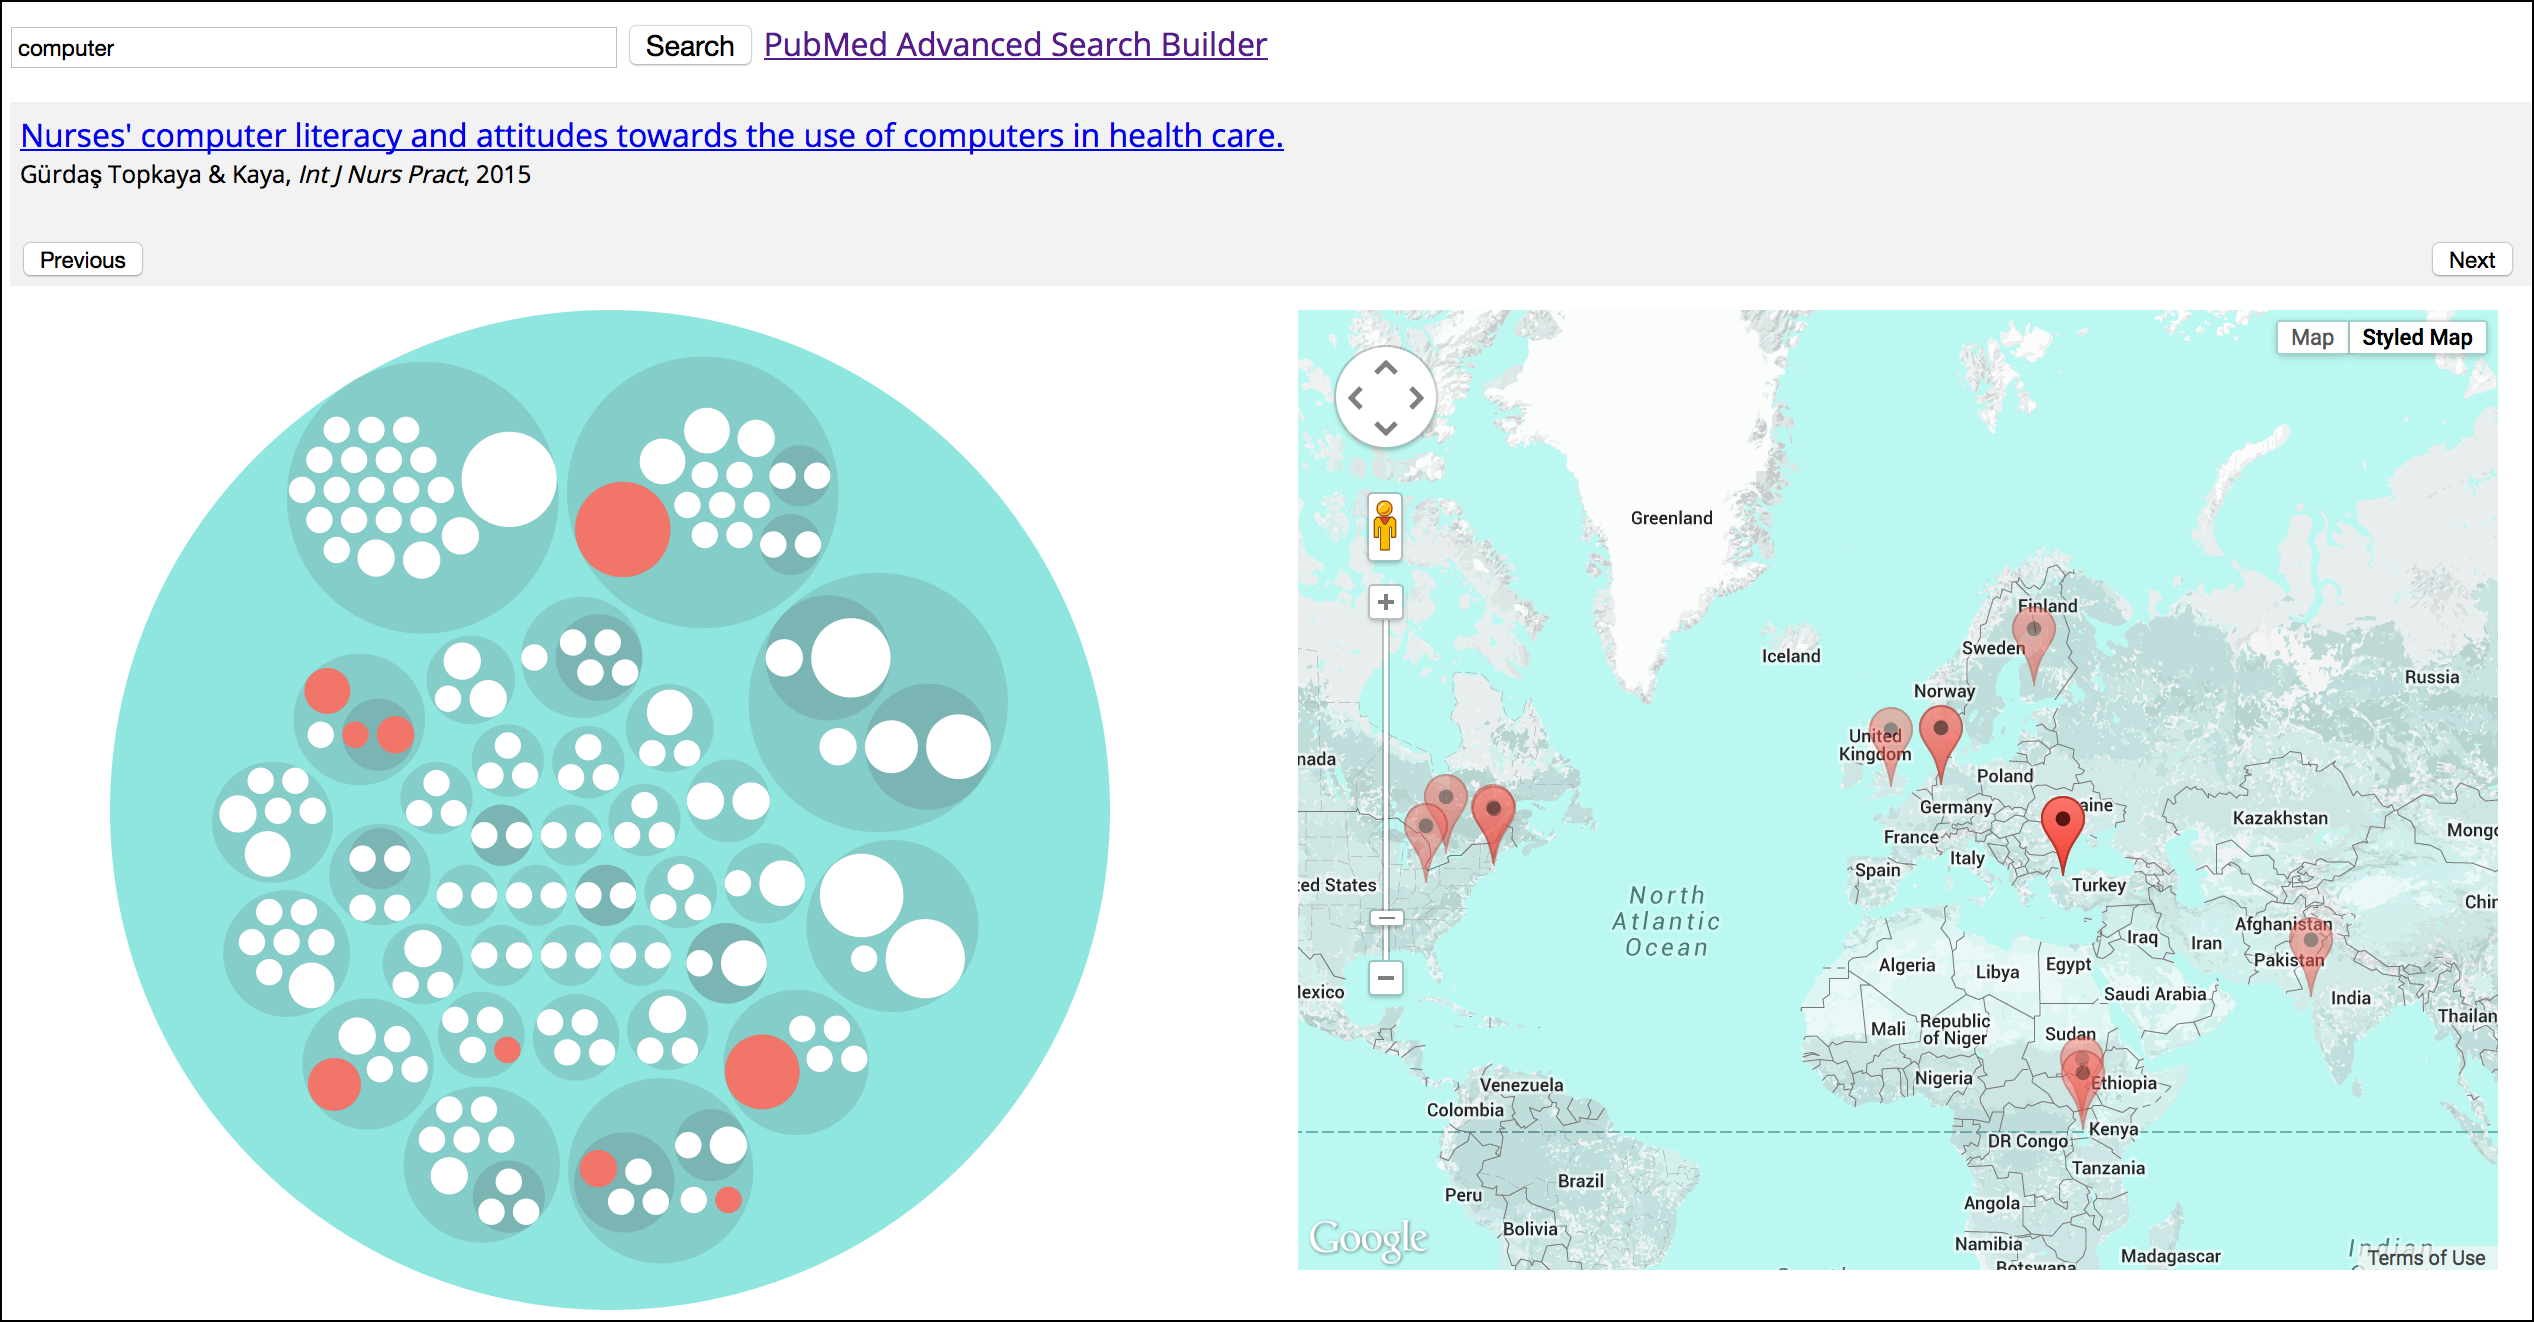
\includegraphics[width=\textwidth]{../lib/images/screen1}
		\subcaption{First result from search term 'computer'.}
	\end{subfigure}\\
	\par\bigskip
	\begin{subfigure}{0.8\textwidth}
		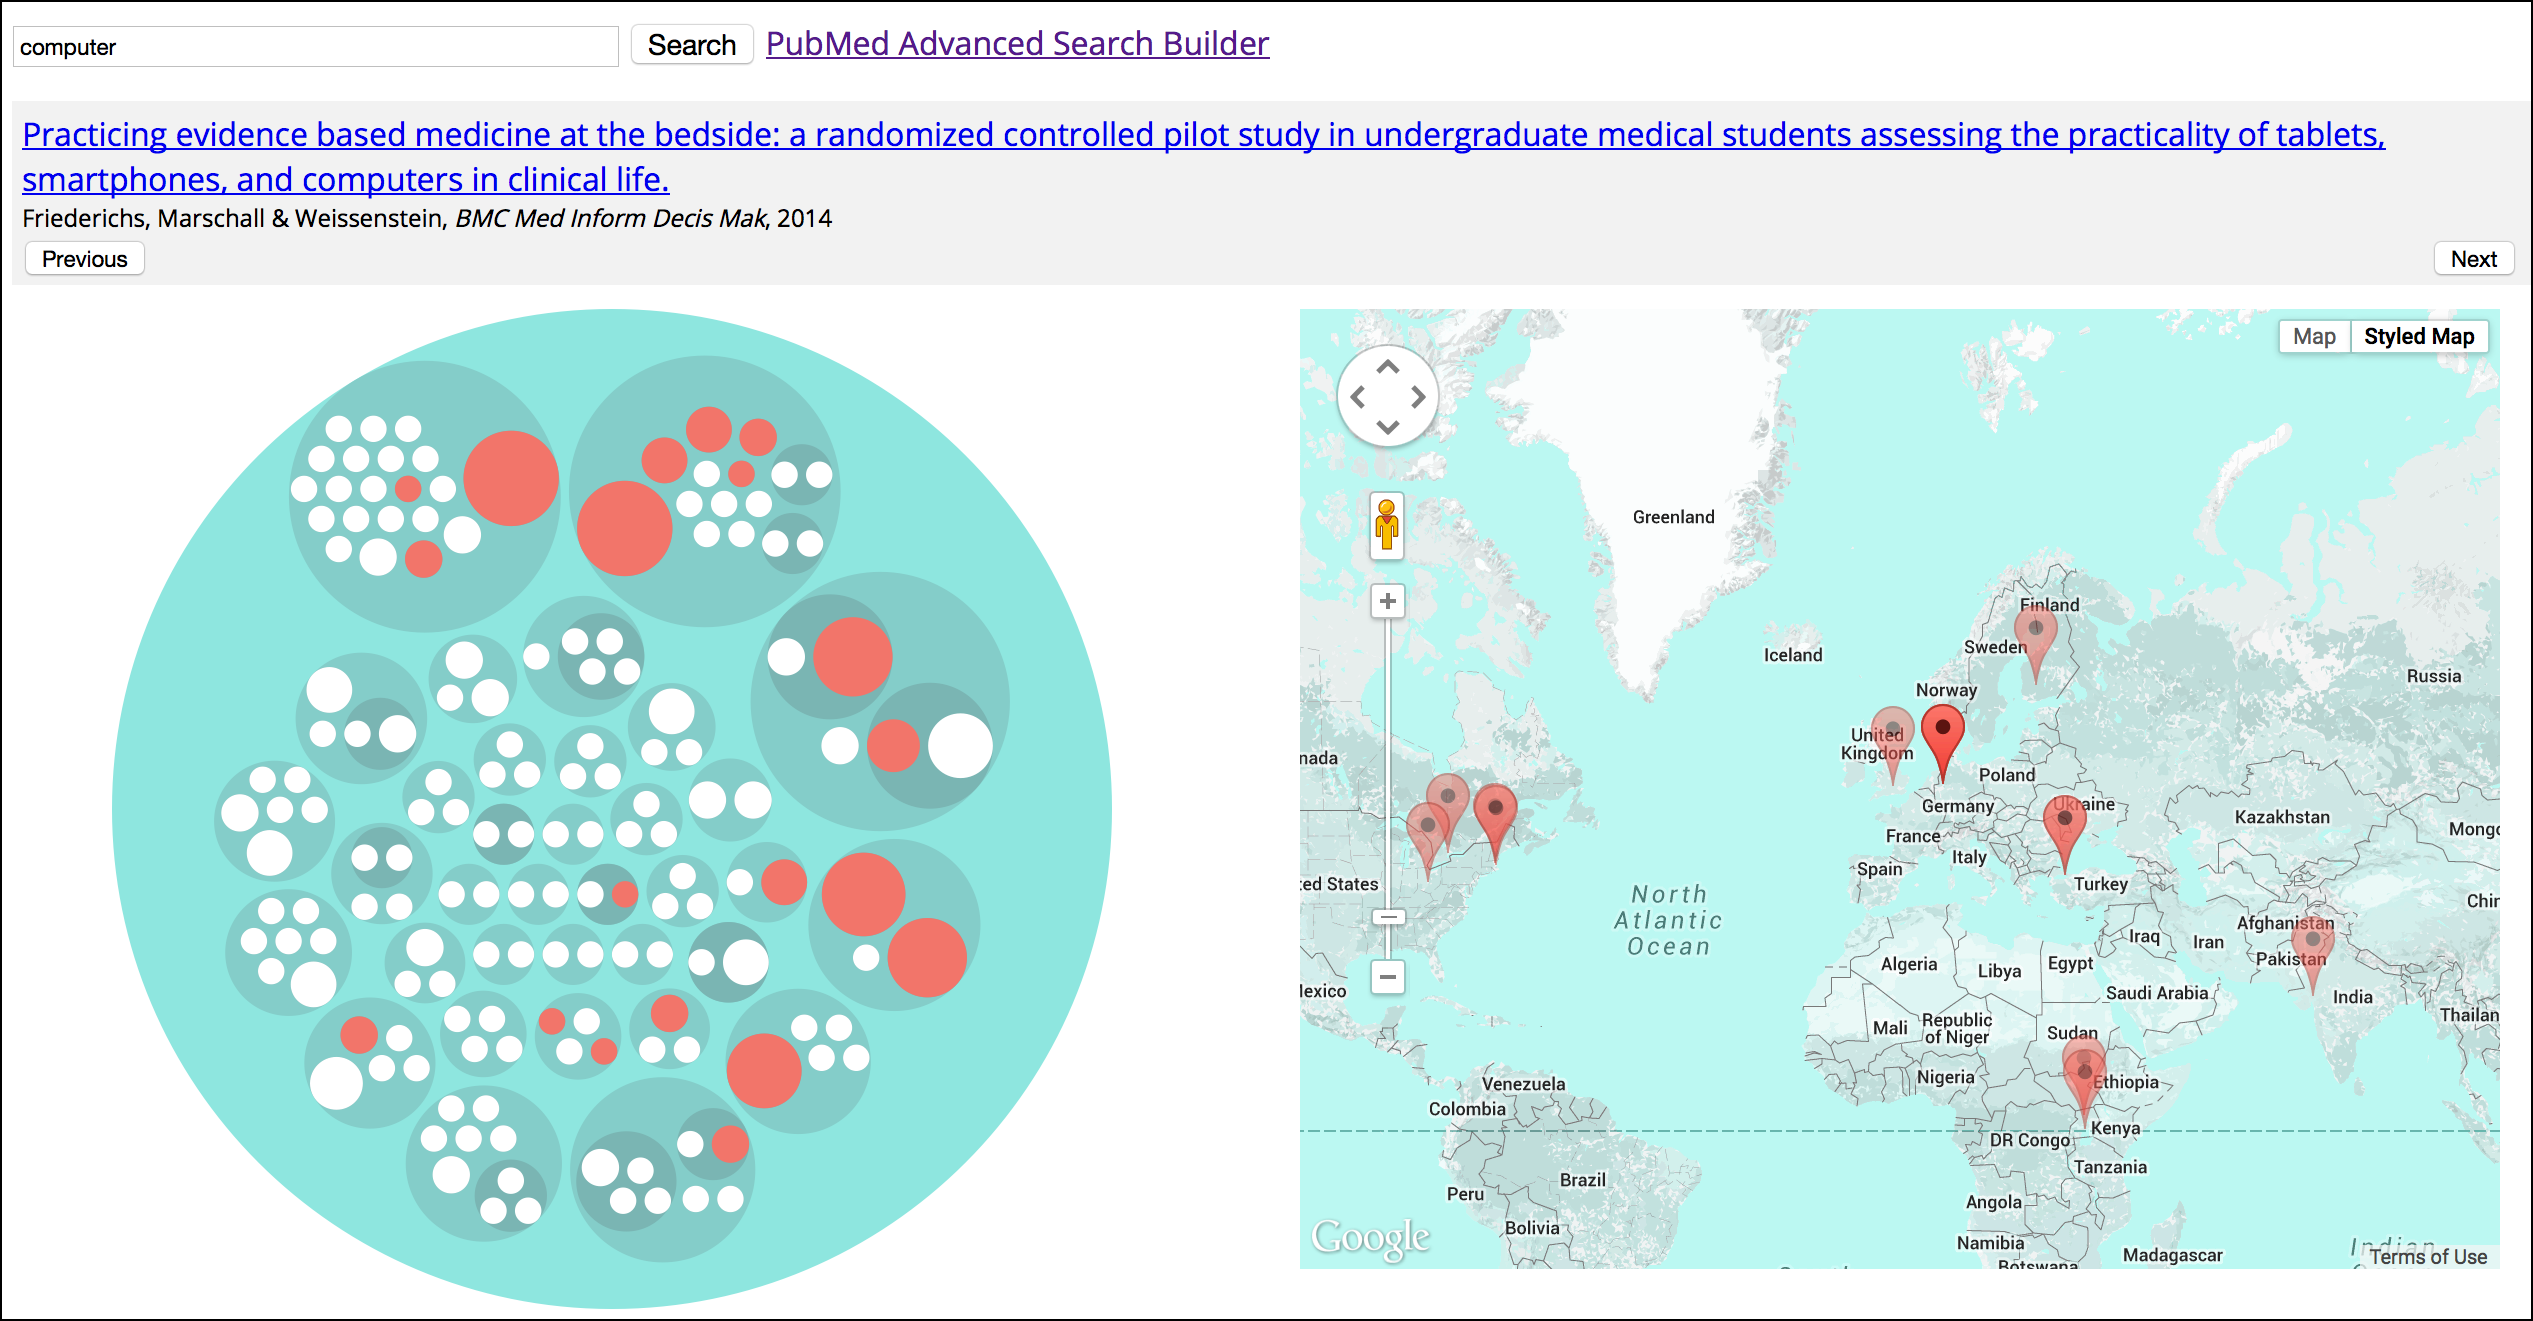
\includegraphics[width=\textwidth]{../lib/images/screen2}
		\subcaption{Second result from search term 'computer'.}
	\end{subfigure}\\
\end{center}
	\begin{subfigure}{0.45\textwidth}
		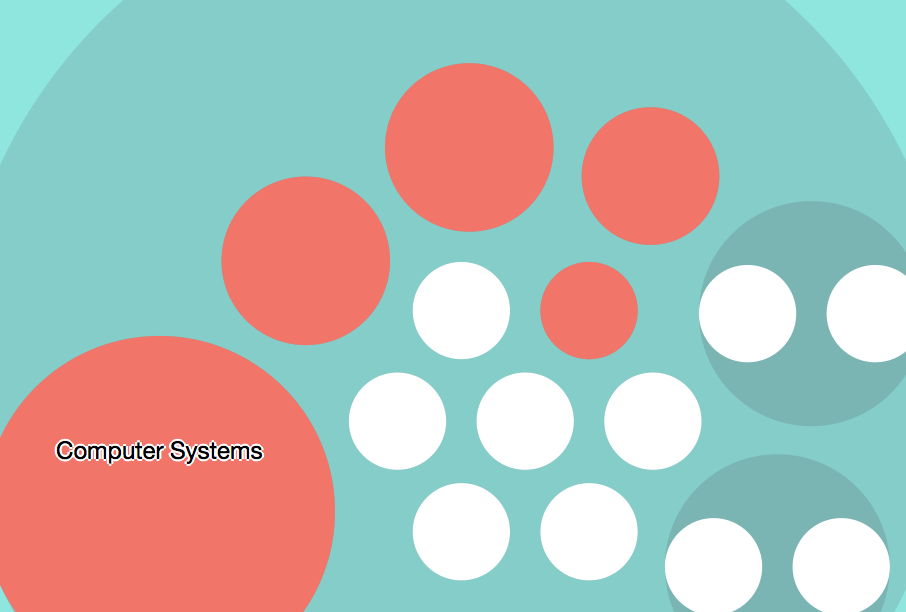
\includegraphics[width=\textwidth]{../lib/images/screen3}
		\subcaption{Text detail and hierarchical organisation.}
	\end{subfigure}%
	\hfill
	\begin{subfigure}{0.45\textwidth}
		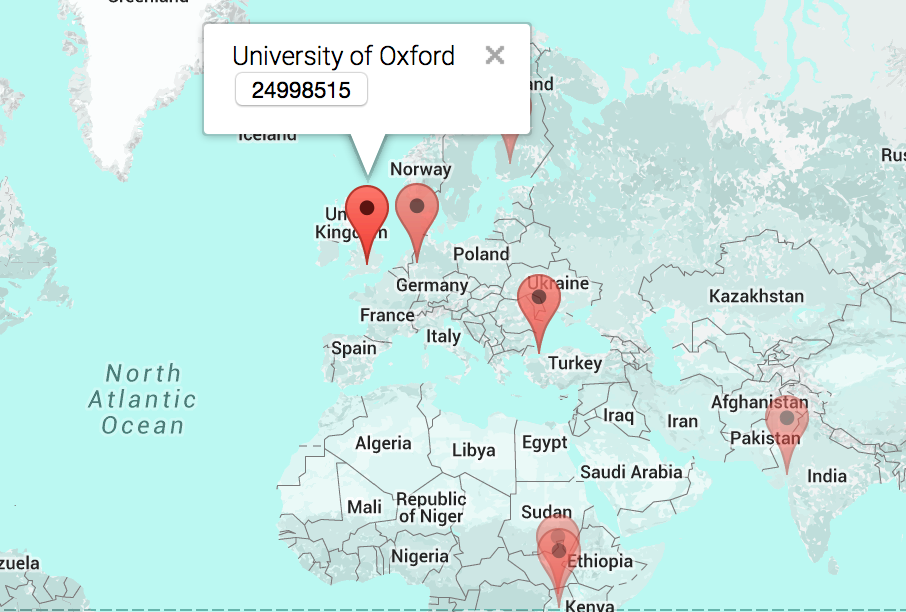
\includegraphics[width=\textwidth]{../lib/images/screen4}
		\subcaption{The map after a marker has been selected.}
	\end{subfigure}\\
\caption{Screenshots from the application.}
\label{fig:screen1}
\end{figure}
\hfill

\section{Architectural features}
\subsection{Design pattern}
The application follows the Model-View-Controller (MVC) software architectural pattern, as is currently common with systems that have an emphasis on interactivity via a graphical user interface. MVC has its origins in Smalltalk applications built in the 1980s when the importance of modularisation was recognised. MVC aims to compartmentalise the logic of the application, the user interface, and the data \cite{mozilla_mvc}.\newline 

\noindent Figure \ref{fig:mvc} shows how the elements of the project align with MVC. The user interacts with elements of the view, in this case a text input form and a graphical button for submission of input to the application. The view specifies the routes through which the data is sent and displayed, as well as the templates for organisation of page content \cite{mozilla_mvc}. The controller receives the input through the web framework and calls functions within the model that can retrieve relevant data based on the search term. After the data processing is complete, it is sent from the controller to the view to generate output for the user. \newline

\noindent The model was focused upon during the development phase of this project, as the efficacy of the view is highly dependent on the quality of the data retrieval and manipulation.\newline

\begin{figure}[!ht]
\begin{center}
	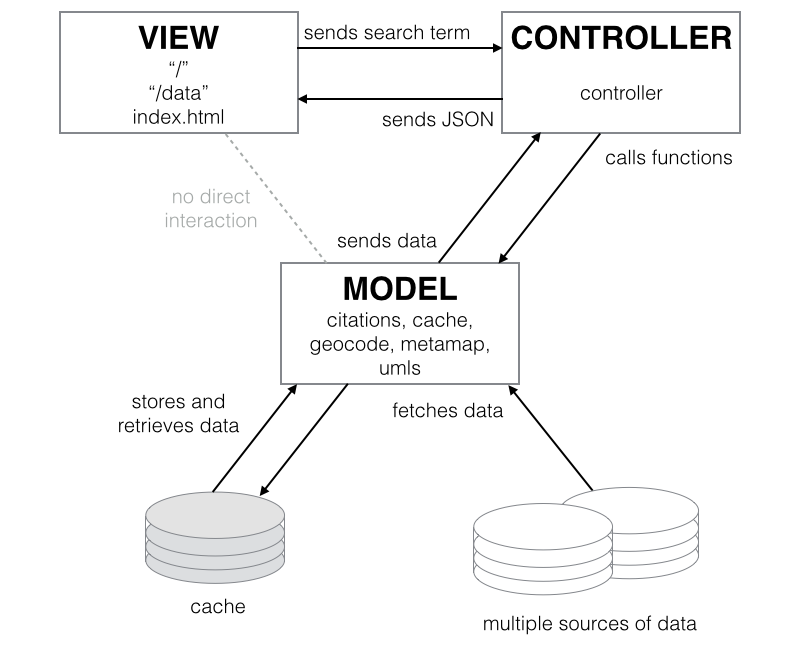
\includegraphics[width=0.7\textwidth]{../lib/images/mvc.png}
	\caption{Diagram to demonstrate fit of the project with the Model-View-Controller software architecture pattern. The routes and HTML template are listed in the View box and the relevant Python modules are listed in the Controller and Model boxes. Each core interaction between the components of the application are displayed next to the directional arrow. The number of data stores are not representative.}
\label{fig:mvc}
\end{center}
\end{figure}
\hfill
\newpage

\subsection{Application flow}
One of the main challenges of the project was to integrate the various programming languages and technologies required along the pipeline, that are each suited to their specific task but not immediately compatible with one another. Figure \ref{fig:flow} is a schematic of the key technologies used for each stage. The general flow of the application processes are described below, and details of each component will be explored in Implementation.

\begin{enumerate}
\item{\textbf{Interaction of the user with the browser}} 
\newline The client side of the web application is presented in a modern browser. A text field is available upon loading of the web page for the user to enter their search term into.
\item{\textbf{Routing via the Flask web framework}}
\newline A GET request is issued from a D3 function to the server via the \texttt{/data} route. The pipeline of data retrieval and manipulation is then started.
\item{\textbf{Retrieving information from papers PubMed}}
\newline The PubMed IDs of up to 20 papers are retrieved from PubMed via a BioPython function \cite{biopython}. First, a cache is queried for any documents with the same PMIDs. Otherwise, the entry is fetched from PubMed using the unique PMID as a reference.
\item{\textbf{Extracting medical concepts from papers}}
\newline The title, abstract, and author keyword fields of PubMed entries are submitted to MetaMap or the MTI, which return a list of concepts.
\item{\textbf{Organising concepts into a semantic hierarchy}}
\newline A local copy of the MetaThesaurus set of vocabularies, organised into a database subset compatible with MySQL, is queried for the concepts as found in the previous step.
\item{\textbf{Assigning locations to affiliate addresses}}
\newline Affiliation addresses are formatted to improve success rates, and then sent to the Google Places API (Application Program Interface) to retrieve a result detailing the geographical coordinates of the most likely result.
\item{\textbf{Adding new documents to the cache}}
\newline PubMed records are inserted into the cache, along with lists of concepts and place IDs for fast repeated retrieval.
\item{\textbf{Data visualisation}}
\newline Data gained from the distinct sources are combined and formatted to send as JSON objects to the client browser. The Google Map and D3 canvases are updated to reflect the semantic and geographical information represented in the data.
\end{enumerate}\newpage

\begin{figure}[!ht]
	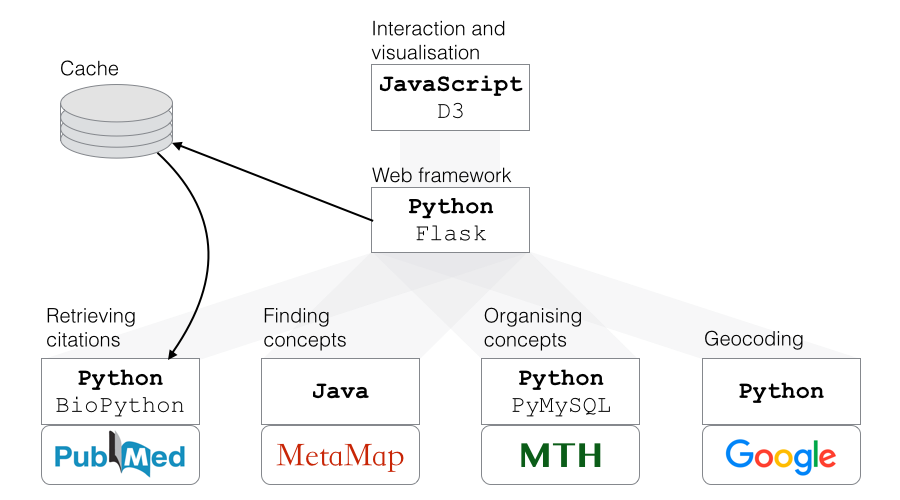
\includegraphics[width=\textwidth]{../lib/images/flow.png}
	\caption{Schematic of the key processes of the system, as explained in the text.}
\label{fig:flow}
\end{figure}

\section{Hardware Requirements}
At this proof-of-concept stage of the application, the server is run locally to the browser. This is mostly due to the storage and processing power used by the local components: MetaMap, and MetaThesaurus via a MySQL server. The MetaThesaurus Release Notes state that a full subset takes up 24.1 GB of disk space \cite{metathesaurus-release}, though the subset used is smaller than this. When uncompressed, MetaMap takes up 14.75 GB of storage space. At least 2 GB of memory is recommended for MetaMap to run \cite{metamap-install}; as MetaMap is a Java application, this is limited by the default maximum heap size of the Java Virtual Machine, which was found to be 2.15 GB on the machine running it. The speed at which MetaMap completes its task is likely affected by the processor speed. It runs in an acceptable time (see chapter 5 for details) using a processor with a clock speed of 2.4 GHz. The MTI utilises multiple servers to parallelise multiple requests but the extent to which individual jobs are parallelised is not known, as it was described as 'likely to be undertaken in the future' in an article published in 2010 by Aronson and Lang at the NIH \cite{metamap2010}.

\end{document}